\section{$n$阶展开方法解双曲正切函数解}
\begin{frame}{$n$阶展开方法解双曲正切函数解}
\begin{enumerate}
\item 双曲正切方法
\item 三类平衡点
\item $n$阶展开多项式的性质
\item 例1: (4+1)Fokas 方程三类平衡点都有
\item 例2: (1+1)EMM 方程第三类平衡点的决定性作用 
\item 例3: 上界的作用
\end{enumerate}
\end{frame}

\begin{frame}{双曲正切方法}
考虑非线性演化方程 
\[
    U\sbrace{u,u\up{1},u\up{2},\cdots}=0, 
\]
其中$u=u(x_1,\cdots,x_d)$, 而$u\up{k}$表示$u$的所有$k$阶导数的集合, 例如$u\up{1}=\bbrace{u_{x_1},\cdots,u_{x_d}}$. 
将
\[
    u=\sum_{k=0}^{m}{a_k\tanh^k(\xi)}
\]
代入原方程后, 方程中各个加法项都是关于$\tanh(\xi)$的多项式, 设他们的次数为 
\[
    s_1 m+d_1,\cdots,s_l m + d_l . 
\]
\end{frame}

\begin{frame}{三类平衡点}
让两个不同的最高项平衡, 可以确定$m$的值. 需要满足:
\begin{itemize}
    \item 整数性: $ m\in \mathbb Z_+$ 
    \item 平衡性: $\exists i\neq j, s_i m+d_i=s_j m+d_j $
    \item 最大性: $\forall k \not\in \bbrace{i,j}, s_i m+d_i\ge s_k m+d_k $
\end{itemize}
\end{frame}

\begin{frame}
\begin{columns}
\begin{column}{.5\textwidth}
\begin{figure}
\centering
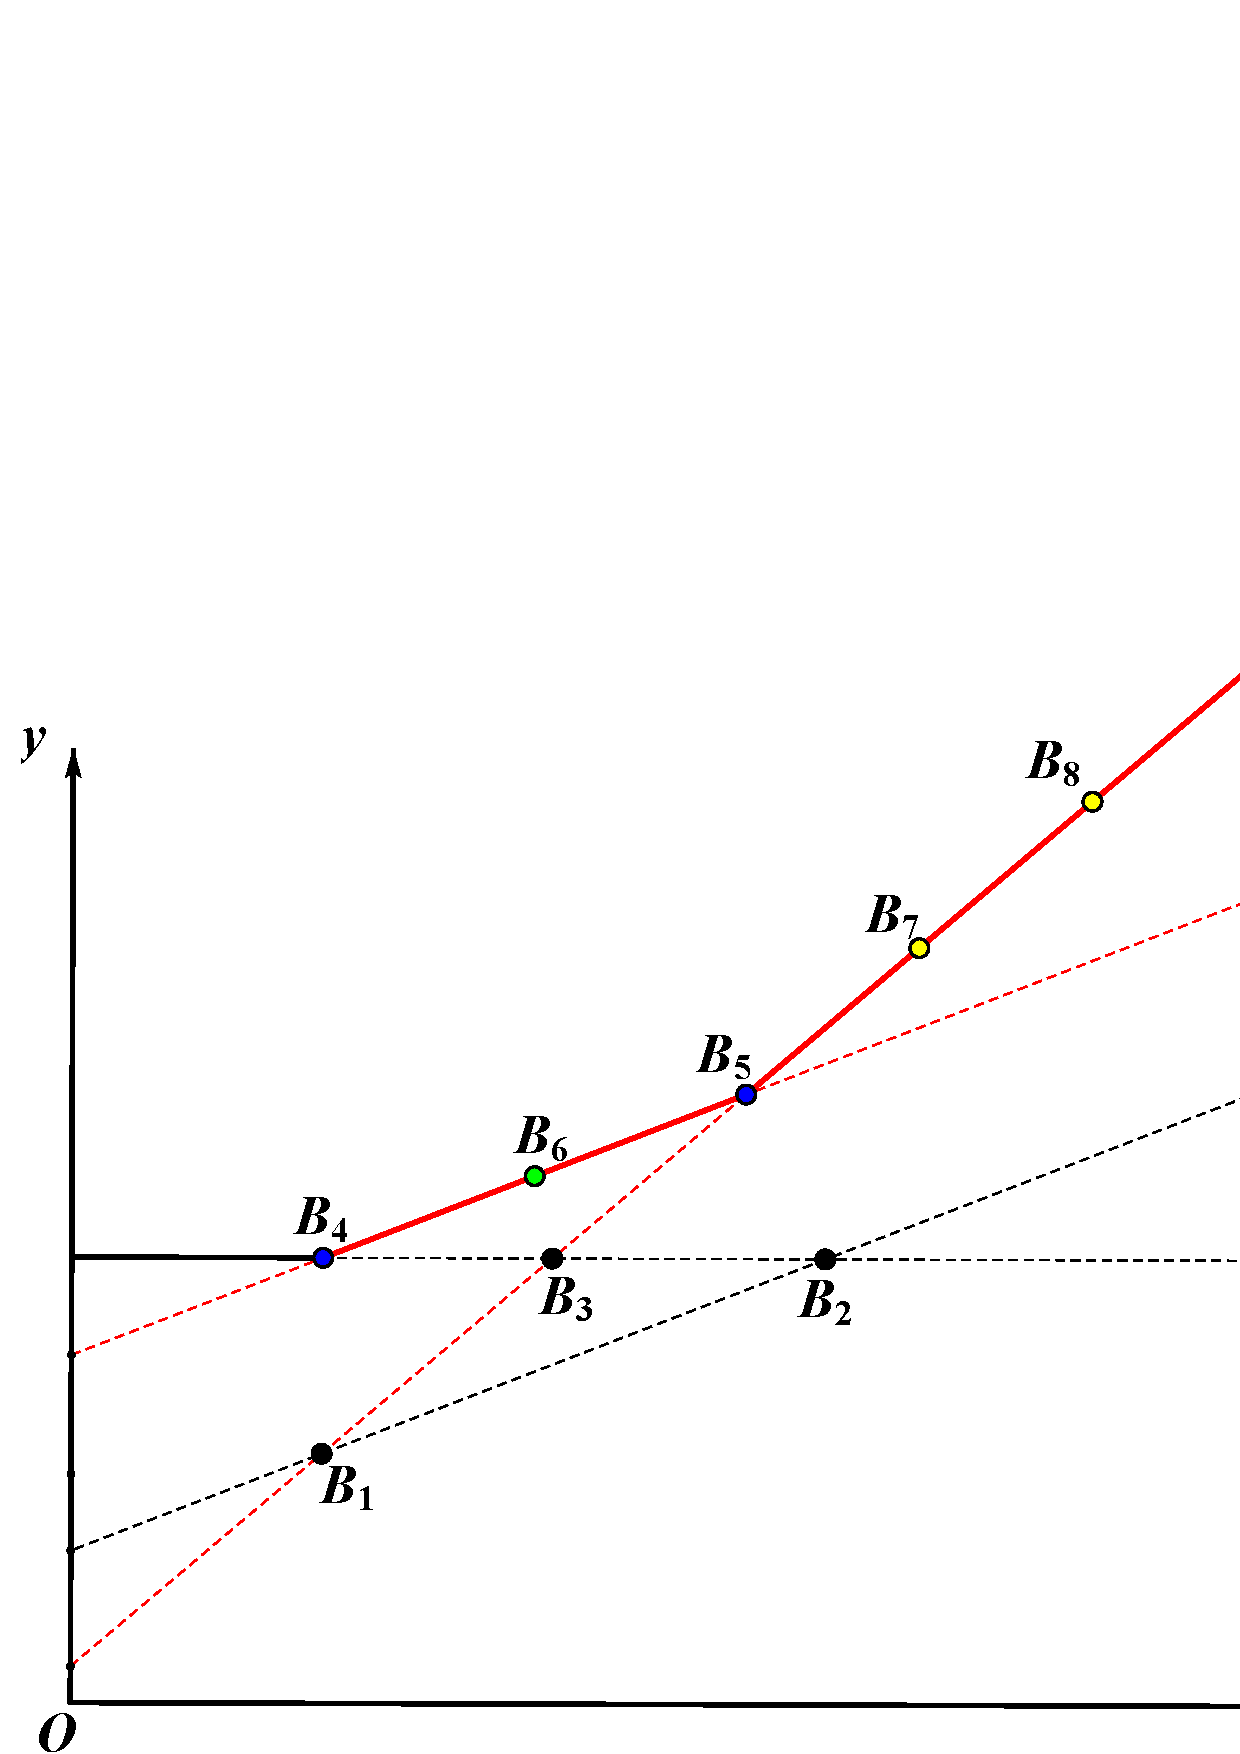
\includegraphics[width=\textwidth]{../paper/fig/ps.pdf}
\caption{平衡点分类示意图}
\end{figure}
\end{column}
\begin{column}{.5\textwidth}
\[
    \lambda_k = s_k m + d_k 
\]
\begin{itemize}
\item $B_1,B_2,B_3$不满足最大性条件, 不是平衡点. 
\item $B_4,B_5$可以由平衡性条件唯一确定, 是\textbf{第一类平衡点}. 
\item $B_6$不能平衡性条件唯一确定, 但是可以由最大性条件确定, 是\textbf{第二类平衡点}.
\item $B_7,B_8$以及右侧的一系列整点, 满足三种平衡条件, 但无法确定其上界, 是\textbf{第三类平衡点}. 我们引入$n$阶展开方法来确定此类平衡点的上界.
\end{itemize}
\end{column}
\end{columns}
\end{frame}

\begin{frame}{$n$阶展开方法}
令$n$阶展开多项式为
\[
    F\sbrace{x,m,u\up n}=\sum_{k=0}^{n-1}{u_k x^{m-k}}+\OO\sbrace{x^{m-n}},
\]
其中 
\[
\OO\sbrace{x^n}=\left\{
\begin{array}{cl}
\text{次数不超过}\,n\,\text{的多项式} & n\ge 0, \\
0                                    & n<0 .
\end{array}
\right.
\]
取
\[
    u=F\sbrace{tanh(\xi),m,a\up{n}}=\sum_{k=0}^{n-1}{a_k \tanh^{m-k}(\xi)}+\OO(\tanh^{m-n}(\xi))
\]
代入原方程, 可以通过最高$n$项的系数来确定第三类平衡点的上界. 
\end{frame}

\begin{frame}{$n$阶展开多项式的性质}
\begin{itemize}
\item $n$阶展开多项式的相乘还是$n$阶展开多项式.
\item $n$阶展开多项式求导后, 其系数中将会包含$m$.
\item $n$阶展开多项式加法的约束条件.
\end{itemize}
\end{frame}

\begin{frame}{乘法}
\[
\begin{split}
& F\sbrace{x,m,u \up n}\cdot F\sbrace{x,l,v\up n} \\
=& \mbrace{\sum_{k=0}^{n-1}{u_k x^{m-k}}+\OO\sbrace{x^{m-n}}}\mbrace{\sum_{k=0}^{n-1}{v_k x^{l-k}}+\OO\sbrace{x^{l-n}}} \\
=& \mbrace{\sum_{k=0}^{n-1}{u_k x^{m-k}}}\mbrace{\sum_{k=0}^{n-1}{v_k x^{l-k}}}+\OO\sbrace{x^{m+l-n}} \\
=& \sum_{p=0}^{n-1}{x^{m+l-p}\mbrace{\sum_{k=0}^p{u_k v_{p-k}}}}+\OO\sbrace{x^{m+l-n}} \\
=& F\sbrace{x,m+l,w\up n} 
\end{split} 
\]
\end{frame}

\begin{frame}{求导}
\[
\begin{split}
& \DIF{t}F\sbrace{x,m,u\up{n}}  \\
=& \DIF{t}\sbrace{\sum_{k=0}^{n-1}{u_k x^{m-k}}+\OO(x^{m-n})} \\
=& \sum_{k=0}^{n-1}{\DIFF{u_k}{t}x^{m-k}}+\DIFF{x}{t}\cdot\sum_{k=0}^{n-1}{u_k (m-k) x^{m-k-1}}+\DIFF{x}{t}\cdot\OO(x^{m-n-1}) \\
=& \sum_{k=0}^{n-1}{\DIFF{u_k}{t}x^{m-k}}+\DIFF{x}{t}\cdot\sbrace{\sum_{k=0}^{n-1}{u_k (m-k) x^{(m-1)-k}}+\OO\sbrace{x^{(m-1)-n)}}} \\ 
=& F\sbrace{x,m,v\up{n}}+\DIFF{x}{t}\cdot F\sbrace{x,m-1,w\up{n}} 
\end{split}
\]
\end{frame}


\begin{frame}{加法}
考虑加法 
\[
    F\sbrace{x,s_i m+d_i,u\up n}+F\sbrace{x,s_j m+d_j,v\up n}
\]
因为我们无法比较$s_i m + d_i$ 和 $s_j m + d_j$ 大小, 所以无法直接求和. 

假设$F\sbrace{x,s_j m+d_j,v\up n}$在求和时不会影响$F\sbrace{x,s_i m+d_i,u\up n}$的前$n$项, 则需 
\[
    s_i m+d_i - n \ge s_j m+d_j 
\]
从而 
\[
\begin{split}
&F\sbrace{x,s_i m+d_i,u\up n}+F\sbrace{x,s_j m+d_j,v\up n} \\
=&\left\{
\begin{array}{cl}
    F\sbrace{x,s_i m+d_i,u\up n} & s_i>s_j,            \\
    F\sbrace{x,s_i m+d_i,w\up n} & s_i=s_j.
\end{array}
\right.
\end{split}
\]
\end{frame}

\begin{frame}{确定第三类平衡点的上界}
\small 
最终, 将$F\sbrace{tanh(\xi),m,a\up{n}}$代入原方程, 可以将原方程重写为$n$阶展开多项式的形式
\[
    F\sbrace{tanh(\xi),\sigma m+\delta,\Omega\up{n}}=0 .
\]
设$\Omega_{k_0}$是第一个非零项, 则: 

(一) $\Omega_{k_0}=0$关于$m$有正整数解, 此时$m$的上界为
\[
    m_{31}=\max\bbrace{m|\Omega_{k_0}=0}.
\]

(二) $\Omega_{k_0}=0$关于$m$没有正整数解, 若加法的假设条件成立, 则原方程无解, 所以需要加法的假设条件不成立才能有解. 此时需要满足 
\[
    \forall s_j<\sigma, \sigma m + \delta - k \le s_j m + d_j
\]
则有
\[
    m\le m_{32} = \underset{s_j<\sigma}{\max}{\frac{d_j-\delta+k}{\sigma-s_j}}
\]
最终, 第三类平衡点的上界为 
\[
    m_3 = \max\bbrace{m_{31},m_{32}}. 
\]
\end{frame}

\begin{frame}{例1: (4+1)Fokas 方程, 含全部三类平衡点}
\small 
对于(4+1)Fokas方程
\begin{equation*}
    u_{tx}-\frac{1}{4}u_{xxxy}+\frac{1}{4}u_{xyyy}+3u_xu_y+3uu_{xy}-\frac{3}{2}u_{wz}=0 ,
\end{equation*}
其阶数列表为$\mbrace{2m+2,m+4,m+4,2m+2,m+2}$. 
\begin{itemize}
\item 首先, 根据$2m+2=m+4$可以得到第一类平衡点$m=2$.
\item 然后, 考虑$m+4=m+4$, 根据最大性约束有$m+4>2m+2$, 可得$m<2$, 所以有第二类平衡点$m=1$.
\item 最后, 因为有两个$2m+2$, 所以需要考虑第三类平衡点. 我们取$\xi=kx+py+qz+rw+ct+\eta$, 代入后可得$n$阶展开的第一个非零项
\begin{equation*}
    \Omega_0 = 24kpa_0^2m\sbrace{m+\frac{1}{2}}. 
\end{equation*}
因为$\Omega_0=0$关于$m$没有正整数解, 所以需要$2m+2\le m+4$, 从而得到第三类平衡点的上界为$m=2$.
\end{itemize}
\end{frame}

\begin{frame}
最终, 我们确定$m=2$, 这既是第一类平衡点, 也是第三类平衡点. \cd{NTCM}给出了原方程的两个解
\begin{equation*}
    \left\{ k=\pm \sqrt {{p}^{2}+{{a}_{2}}},{{a}_{0}}=-\frac{2\,{{a}_{2}}}{3}-\frac{c}{3\,p}+ \frac{q\,r}{2\,k\,p},{{a}_{1}}=0\right\} .
\end{equation*}
\end{frame}

\begin{frame}{例2: (1+1)EMM 方程, 第三类平衡点的决定性作用}
考虑方程
\begin{equation*}
    {{u}_{t}}+{{u}_{x}}+\alpha\,{{u}_{xxx}}+\beta\,u\,{{u}_{x}}+\gamma\,u\,{{u}_{xxx}}+\delta\,{{u}_{x}}\,{{u}_{xx}}=0,
\end{equation*}
这是一个从弹性介质的微观结构中导出的非线性演化方程, 其阶数列表为$[m+1,m+1,2m+1,2m+3,2m+3]$, 只可能存在第三类平衡点.  取$\xi=kx+ct+\eta$, 由
\begin{equation*}
    \Omega_0=-{{{a}_{0}}}^{2}\,{k}^{3}\,m\,\left( m+1\right) \,\left( m\,\delta+\gamma\,m+2\,\gamma\right)
\end{equation*}
可得 $m=0$, 原方程没有非平凡的解. 当$m=\frac{-2 \gamma}{\gamma+\delta}$为正整数时, 就存在其它可能的平衡点.
\end{frame}

\begin{frame}
当$\gamma=-1,\delta=3$时, $m=1$, 原方程有两个解 
\begin{equation*}
    \bbrace{a_0=\alpha,k=\pm\frac{\sqrt{\beta}}{2},c=-k\frac{\alpha \beta+1}{2},a_1=a_1}.
\end{equation*}

此外, 我们总结出: 当$n\ge 1$时, 若$\gamma=-n,\delta=n+1$, 则$m=2n$, 原方程有解 
\begin{equation*}
u=(-1)^n a_{2n} \sbrace{\tanh^2\sbrace{\frac{\pm\sqrt{-\beta}}{2n}x-\frac{\pm\sqrt{-\beta}(\alpha\beta+n)}{2n^2}t+\eta}-1}^n+\frac{\alpha}{n} .
\end{equation*}
\end{frame}